% !TeX root = ../introduction.tex
\subsection{Neural Networks}\label{sec:introduction:neural-networks}

Much of the future discussion on neural network language models will require at least an intuitive understanding of neural networks.
This section aims to provide enough background and vocabulary to facilitate discussion of neural networks as a concept without becoming bogged down in a nontrivial amount of detail.
\begin{figure}[h]
    \centering
    
\includegraphics[scale=0.5]{machine_learning}
    \caption{The pile gets soaked with data and starts to get mushy over time, so it's technically recurrent \cite{xkcd_machine_learning}}\label{fig:neural-networks:xkcd-machine-learning}
\end{figure}
There are many other excellent introductions to neural networks that provide much more detail such as \cite{goodfellow_bengio_courville_2016} for a general mathematical treatment, or \cite{goldberg_2017} for a treatment specific to processing natural language.
\TODO{This information is provided purely to ensure a consistent vocabulary, and has been produced without reference material. It should be fact-checked and appropriately cited.}

\subsubsection{A Biological Metaphor}\label{sec:neural-networks-biological-metaphor}

If our intent is to produce intelligent, sophisticated statistical models, it is useful to motivate our model with the biological metaphor of a single neuron.
Of course, our intent is not to emulate, nor is it to simulate a collection of biological neurons.
We simply wish to motivate a mathematical discussion of a statistical model that has proved useful in data analysis, modeling, and prediction.
In this spirit, we note that it is well beyond the scope of this paper to provide a biologically correct description of the hugely complex field of neuroscience.
In fact, it would be reasonable to present neural networks devoid of any biological motivation simply as a mathematical model that has proven to be useful.
\begin{figure}[h]
    \centering
    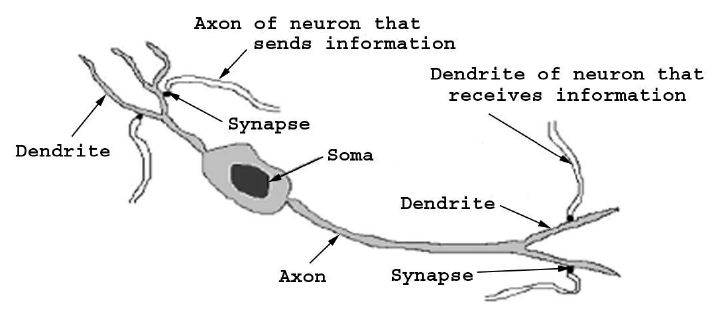
\includegraphics[scale=0.5]{biological_neuron}
    \caption{A biological neuron \cite{bio_neuron}}\label{fig:neural-networks:biological-neuron}
\end{figure}
\autoref{fig:neural-networks:biological-neuron} shows a ``typical'' neuron (of course there is no such thing) with various labeled components.
In the most general sense, a neuron takes electrical stimulation through its dendrites, processes the received information, and under the right conditions emits a signal through its axon to the dendrites of an adjacent neuron \cite{bio_neuron}.
Somehow, through an organization of many such neurons, intelligent behavior emerges \cite{castro_2006}.

\subsubsection{An Artificial Neuron}\label{sec:neural-networks:artificial-neuron}

Even such a grossly simplified treatment of a neuron provides motivation for the artificial neuron shown in \autoref{fig:neural-networks:artificial-neuron}.
\begin{figure}[h]
    \centering
    \begin{tikzpicture}[
        node distance=3cm,
        >={Stealth[length=2mm]},
        ]

        \node[draw, circle, label=below:{activation}] (unit) {$\sum\quad f$};
        \draw[dashed] (unit.north) -- (unit.south);

        \node[draw, circle, above left=2.1cm of unit] (x_0) {$x_0$};
        \node[draw, circle, below=5mm of x_0] (x_1) {$x_1$};
        \node[draw, circle, below=5mm of x_1] (x_2) {$x_2$};
        \node[below=1mm of x_2] (dots) {$\vdots$};
        \node[draw, circle, below=3mm of dots, label=below:{input}] (x_n) {$x_n$};

        \node[draw, circle, right=3cm of unit, label=below:{output}] (output) {$y$};

        \draw[->] (x_0) -- node[midway, sloped, above] {$w_0$} (unit);
        \draw[->] (x_1) -- node[midway, sloped, above] {$w_1$} (unit);
        \draw[->] (x_2) -- node[midway, sloped, above] {$w_2$} (unit);
        \draw[->] (x_n) -- node[midway, sloped, above] {$w_n$} (unit);
        \draw[->] (unit) -- node[midway, above] {$f\left(\sum_{i=1}^n w_ix_i \right)$} (output);

    \end{tikzpicture}
    \caption{An artificial neuron}\label{fig:neural-networks:artificial-neuron}
\end{figure}
The artificial neuron, called a \textit{unit}, takes a fixed number of inputs $x_0, \dots, x_n$, multiplies each with its corresponding weight, and adds the weighted inputs together before piping the result through the activation function $f$.
Note that if the inputs are treated as a column vector $\vec x$, and the weights as a vector $\vec w$, the output is the result of the operation $y = f(\vec w \cdot \vec x)$.

Often it is useful to add a bias term $b$
\begin{equation}
    y = f(\vec w \cdot \vec x + b) \label{eq:neural-networks:ffnn-unit}
\end{equation}
by adding a fixed unitary input to the neuron as in \autoref{fig:neural-networks:artificial-neuron-bias}.
This allows us to treat the bias term exactly like one of the weights when assembling multiple such units together to form a network.
\begin{figure}[h]
    \centering
    \begin{tikzpicture}[
        node distance=3cm,
        >={Stealth[length=2mm]},
        ]

        \node[draw, circle, label=below:{activation}] (unit) {$\sum\quad f$};
        \draw[dashed] (unit.north) -- (unit.south);

        \node[draw, circle, above left=2.1cm of unit] (one) {$+1$};
        \node[draw, circle, below=5mm of one] (x_0) {$x_0$};
        \node[draw, circle, below=5mm of x_0] (x_1) {$x_1$};
        \node[below=1mm of x_1] (dots) {$\vdots$};
        \node[draw, circle, below=3mm of dots, label=below:{input}] (x_n) {$x_n$};

        \node[draw, circle, right=3cm of unit, label=below:{output}] (output) {$y$};

        \draw[->] (one) -- node[midway, sloped, above] {$b$} (unit);
        \draw[->] (x_0) -- node[midway, sloped, above] {$w_0$} (unit);
        \draw[->] (x_1) -- node[midway, sloped, above] {$w_1$} (unit);
        \draw[->] (x_n) -- node[midway, sloped, above] {$w_n$} (unit);
        \draw[->] (unit) -- node[midway, above] {$f(\vec w \cdot \vec x + b)$} (output);

    \end{tikzpicture}
    \caption{An artificial neuron with a unitary bias input}\label{fig:neural-networks:artificial-neuron-bias}
\end{figure}

\subsubsection{Assembling Neurons into Networks}\label{sec:neural-networks:assembling-neurons}

Presumably then, the intelligence of a neural network has something to do with how the units are assembled together, and with the magical weight values associated with each unit.
Unlike the chaotic and organic layout in the human body, we assemble the artificial neurons into sequential layers, and connect the outputs of the previous layer to the inputs of the next.

\begin{figure}[h]
    \centering
    \begin{tikzpicture}[scale=1.8, >={Stealth[length=2mm]},->, draw=black!50, node distance=3cm]
        \tikzstyle{every pin edge}=[<-]
        \tikzstyle{neuron}=[draw, black, thick, circle, minimum size=1cm, inner sep=0pt]
        \tikzstyle{annot} =[text width=4em, text centered]

        % Draw the input layer nodes
        \foreach \name / \y in {0,...,3}
        \node[neuron, pin=left:{$x_\y$}] (I-\name) at (0,-\y-1) {};

        % Draw the hidden layer nodes
        \foreach \name / \y in {1,...,5}
        \path[yshift=0.5cm]
        node[neuron] (H-\name) at (2.5cm,-\y cm) {};

        % Draw the output layer node
        \node[neuron,pin={[pin edge={->}]right:{$y$}}, right of=H-3] (O) {};

        % Connect every node in the input layer with every node in the hidden layer.
        \foreach \source in {0,...,3}
        \foreach \dest in {1,...,5}
        \path (I-\source) edge (H-\dest);

        % Connect every node in the hidden layer with the output layer
        \foreach \source in {1,...,5}
        \path (H-\source) edge (O);

        % Annotate the layers
        \node[annot,above of=H-1, node distance=1cm] (hl) {Hidden layer};
        \node[annot,left=2.5cm of hl] {Input layer};
        \node[annot,right of=hl] {Output layer};
    \end{tikzpicture}
    \caption{Multiple units arranged into a network}\label{fig:neural-networks:multilayer-perceptron}
\end{figure}

When we treat the cells as a vertical layer, \autoref{eq:neural-networks:ffnn-unit} becomes
\begin{equation}
    \vec y = f(W^T \vec x + \vec b) \label{eq:neural-networks:ffnn-layer}
\end{equation}
where each of the weight vectors $\vec w$ for each cell is arranged into the matrix $W$, and each of the $y$-values are concatenated to form $\vec y$.
Common choices for the activation function $f$ are the hyperbolic tangent, sigmoid, rectified linear unit, and softmax functions.
Note that the use of $f$ in \autoref{eq:neural-networks:ffnn-layer} assumes that the same activation function is used for every unit in the layer.

Due to the large amount of homogeneity in the units for each layer, we almost never draw schematic diagrams of a network's architecture showing the individual units.
Instead, we treat the layer of units as the basic abstraction as in \autoref{fig:neural-networks:architecture}.
\begin{figure}[h]
    \centering
    \begin{tikzpicture}[
        node distance=2.6cm,
        >={Stealth[length=2mm]},
        layer/.style={draw, minimum width=1cm},
        input/.style={draw, dashed, minimum height=1cm, minimum width=0.8cm}
        ]

        \node[input] (x_0) {$x_0$};
        \node[input, below=1mm of x_0, anchor=north] (x_1) {$x_1$};
        \node[below=3mm of x_1, anchor=north] (ellipsis) {$\vdots$};
        \node[input, below= 3mm of ellipsis, anchor=north] (x_n) {$x_{n_1}$};

        \node[left=1cm of x_0] (x_0_label) {$x_0$};
        \node[left=1cm of x_1] (x_1_label) {$x_1$};
        \node[left=1cm of x_n] (x_n_label) {$x_{n_1}$};

        \node[layer, fit={(x_0) (x_1) (ellipsis) (x_n)}, label=below:{$\vec x$}, label=above:{$n_1$}] (input) {};

        \node[layer, label=below:{$\tanh$}, label=above:{$n_2$}, right of=input, minimum height=4cm] (hidden) {};
        \node[layer, label=below:{softmax}, label=above:{$n_3$}, right of=hidden, minimum height=7cm] (softmax) {};
        \node[right=1.2cm of softmax] (output) {$\vec y$};

        \draw[->] (x_0_label) -- (x_0);
        \draw[->] (x_1_label) -- (x_1);
        \draw[->] (x_n_label) -- (x_n);

        \draw[->] (input) -- node[midway, above]{$W_1$} (hidden);
        \draw[->] (hidden) -- node[midway, above]{$W_2$} (softmax);
        \draw[->] (softmax) -- (output);
    \end{tikzpicture}
    \caption{An example neural network architecture diagram}\label{fig:neural-networks:architecture}
\end{figure}
The dimension of each layer is shown at the top of each layer, and the activation function of the non-input layers is indicated below each layer.
The underlying mathematical operation that this architecture defines is
\begin{equation*}
    \vec y = \softmax\left(W_2^T \tanh(W_1^T \vec x + \vec{b_1}) + \vec{b_2}\right)
\end{equation*}
where $\vec{b_1}$ and $\vec{b_2}$ are the implicit bias vectors, and $W_1$ and $W_2$ are the weight matrices for the $\tanh$ and $\softmax$ layers respectively.

Here, the softmax activation function
\begin{equation}
    \softmax(\vec x) = \frac{\exp\left(\vec x\right)}{\sum\exp\left(\vec x\right)} \label{eq:neural-networks:softmax}
\end{equation}
is applied element-wise to the vector $\vec x$, and produces the vector $\vec y$ which can be treated as a probability distribution over $n$ values.
That is, the vector $y$ sums to 1.
The softmax activation function is often used in neural networks whose output is to be treated as a probability, and will be used extensively in language modeling.

\TODO{Add a \textit{brief} discussion on datasets, objective functions, and optimization methods.}
\TODO{See also \cite{eisenstein_2019} for a brief but rigorous mathematical introduction to neural networks.}
